\chapter{Methodology, Implementation and Experimental Results}
\label{chap:implementation}

The first experiment focus on the beacons data directly. It aims to calibrate the meta-parameters and analyzes the precision of the distance estimation between the phone and the beacons. The experiment take place in a corridor, with no obstacle and a direct Line of Sight (LoS) between the phone and the sensors. The sensor is placed at 1.5 meters from the ground and measurements are taken at every meter, starting at "0" ($L_0$), with the phone touching the sensor, and up to 15 meters away from it ($L_{15}$). At each step, the phone take measurements for 20 seconds. Each sensor is tested with no other sensor active at the same time.

\begin{figure}[H]
    \centering
    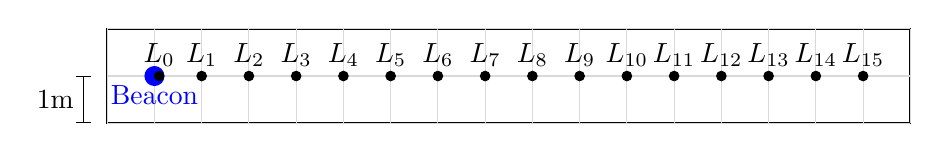
\begin{tikzpicture}[scale=0.6]
        % Room dimensions 
        \draw[thick] (0,0) rectangle (17,2);  
        % Grid (optional, for reference)
        \draw[gray!30, step=1] (0,0) grid (17, 2);
        
        % ESP32 devices (blue dots)
        \filldraw[blue] (1, 1) circle (0.2) node[below] {Beacon};

        % User positions (X marks)
        \filldraw (1.1, 1) circle (0.1) node[above] {$L_0$};
        \filldraw (2, 1) circle (0.1) node[above] {$L_1$};
        \filldraw (3, 1) circle (0.1) node[above] {$L_2$};
        \filldraw (4, 1) circle (0.1) node[above] {$L_3$};
        \filldraw (5, 1) circle (0.1) node[above] {$L_4$};
        \filldraw (6, 1) circle (0.1) node[above] {$L_5$};
        \filldraw (7, 1) circle (0.1) node[above] {$L_6$};
        \filldraw (8, 1) circle (0.1) node[above] {$L_7$};
        \filldraw (9, 1) circle (0.1) node[above] {$L_8$};
        \filldraw (10, 1) circle (0.1) node[above] {$L_9$};
        \filldraw (11, 1) circle (0.1) node[above] {$L_{10}$};
        \filldraw (12, 1) circle (0.1) node[above] {$L_{11}$};
        \filldraw (13, 1) circle (0.1) node[above] {$L_{12}$};
        \filldraw (14, 1) circle (0.1) node[above] {$L_{13}$};
        \filldraw (15, 1) circle (0.1) node[above] {$L_{14}$};
        \filldraw (16, 1) circle (0.1) node[above] {$L_{15}$};
        
        % Scale indicator
        \draw[|-|] (-0.5,0) -- (-0.5,1) node[midway, left] {1m};
    \end{tikzpicture}
    \caption{Experimental setup for the first experiment showing three ESP32 devices and a single POI with its detection radius.}
    \label{fig:exp1_setup}
\end{figure}

\section{Calibration}

The \autoref{eq:BLE_RSSI} to derive the distance from the Received Signal Strength Indicator (RSSI) has two meta parameters. The first one is the $tx_{power}$, which is equivalent to the RSSI at one meter. The second is the environmental factor ($N$) and depends of the layout of the surrounding environment. 


Experimental results in \autoref{fig:beacon-rssi-1m} show that the distribution of $tx_{power}$ is quite instable, while still close to the mean. The best values can be calculated using the mean of the values for each beacon. As we  can see, while it's close to the theoretical value of $-69$, it's a little bit lower, and even well lower for the third beacon, at $-63$.

\begin{figure}[h]
    \centering
    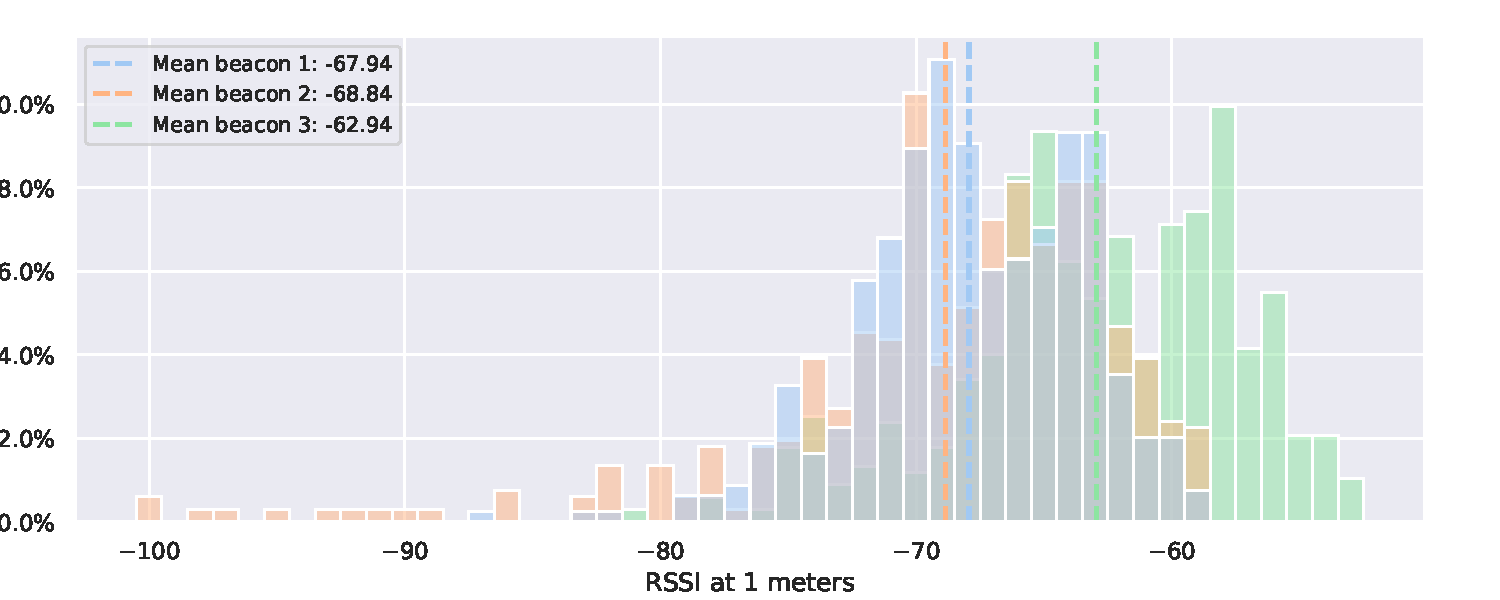
\includegraphics[width=\linewidth]{assets/beacon-rssi-1m.pdf}
    \caption{Variation in RSSI relative to Distance from Beacons}
    \label{fig:beacon-rssi-1m}
\end{figure}

The environmental factor ($N$) typically range from $2$ in almost perfect environments to $4$ in very crowded environments. The experimental data shown in \autoref{fig:beacon-environmental-factor} have been taken with LoS in an almost-perfect environment of a corridor. As we can see, the best match happens for $N=2$ for each beacon, with a relatively low Median Absolute Deviation (MAD). The MAD is preferred here has the logarithmic effect can significantly higher the mean and make it unusable.

\begin{figure}[h]
    \centering
    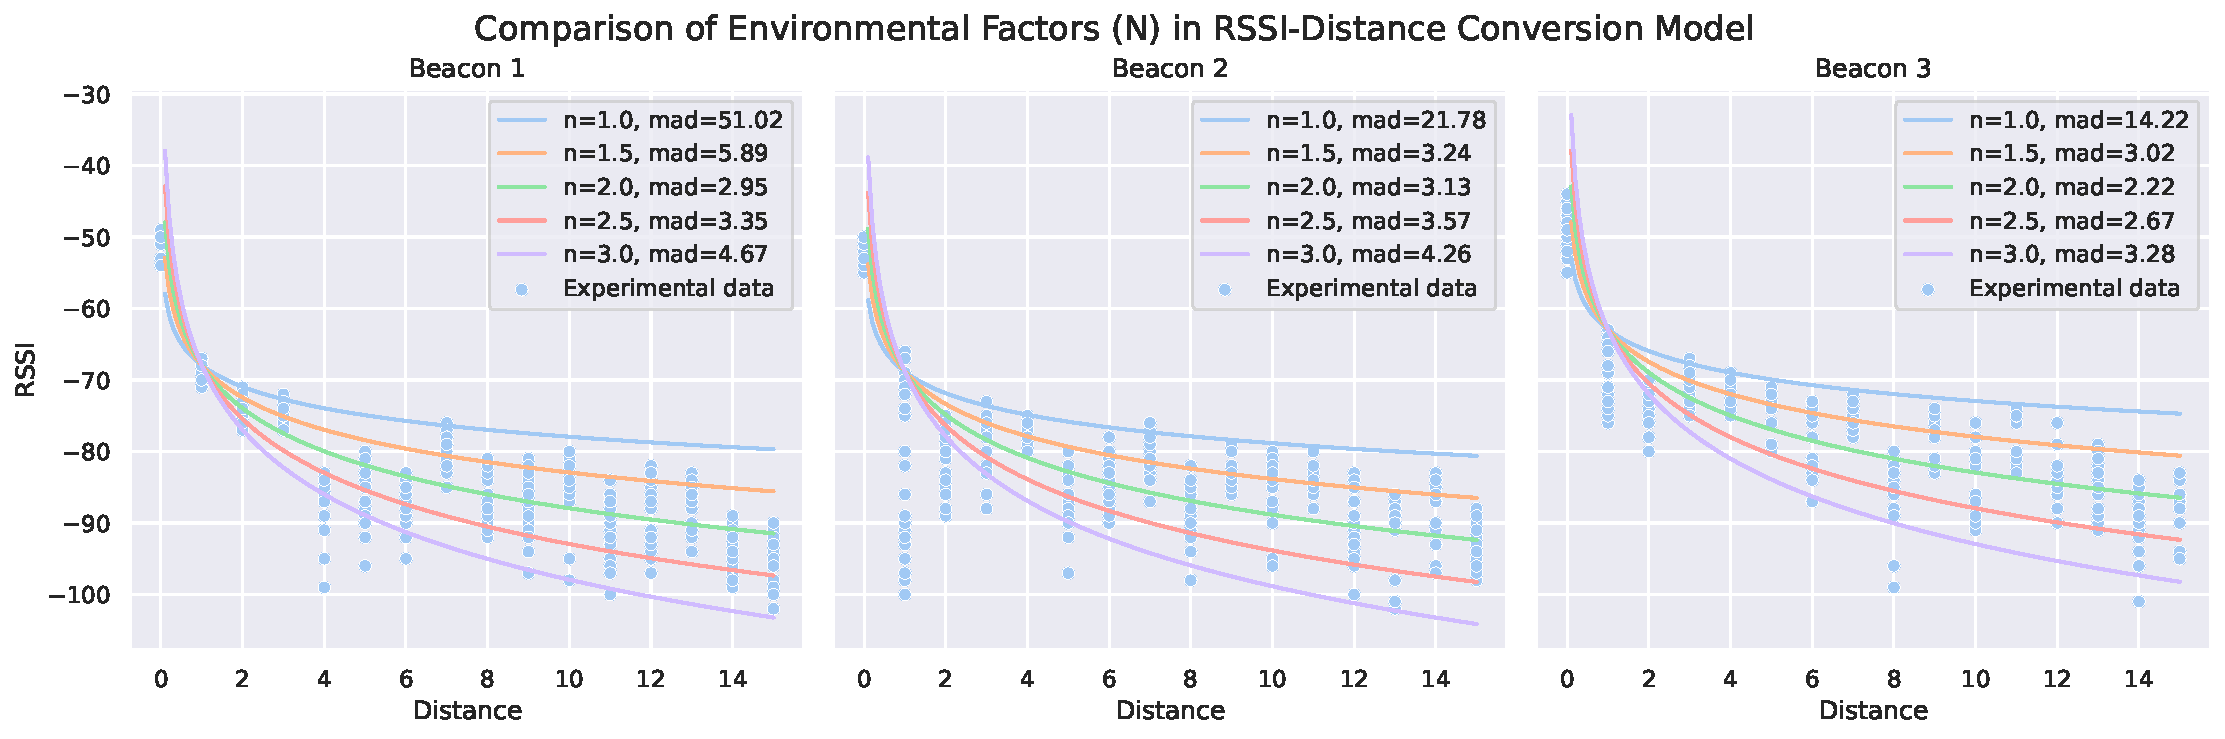
\includegraphics[width=\linewidth]{assets/beacon-environmental-factor.pdf}
    \caption{Comparison of the environmental factors (N)}
    \label{fig:beacon-environmental-factor}
\end{figure}

Theses findings show that during the calibration phase, each beacon must be evaluated individually to determine it's $tx_{power}$ but this value should remain the same even after a change of the environment. Then the environmental factor $N$ must be evaluated for the environment, but remains the same for each beacon, significantly reducing the preparation work.

\section{Distance to beacons}

Experimental results of the variation of the raw distance error relative to the distance to beacons presented in \autoref{fig:beacon-dist-raw-error} confirms the findings of \cite{spachos_ble_2020}, where there is a corelation between the precision and the distance of the beacons. Also, close beacons up to a few meters leads to very low error and small range.

We can see that the median error for raw distances are between 2 and 3 meters, 75\% of the errors are below 5 meters, and 90\% below 8 meters.

% How did I choose the parameters? Which ones?

 \autoref{fig:beacon-dist-filtered-error} present the results once the Kalman filter is applied, reducing the medians between 1.5 and 2.5 meters, 75\% of the errors bellow 4 meters but keep the 90\% around 8 meters. 

\begin{figure}[h]
    \centering
    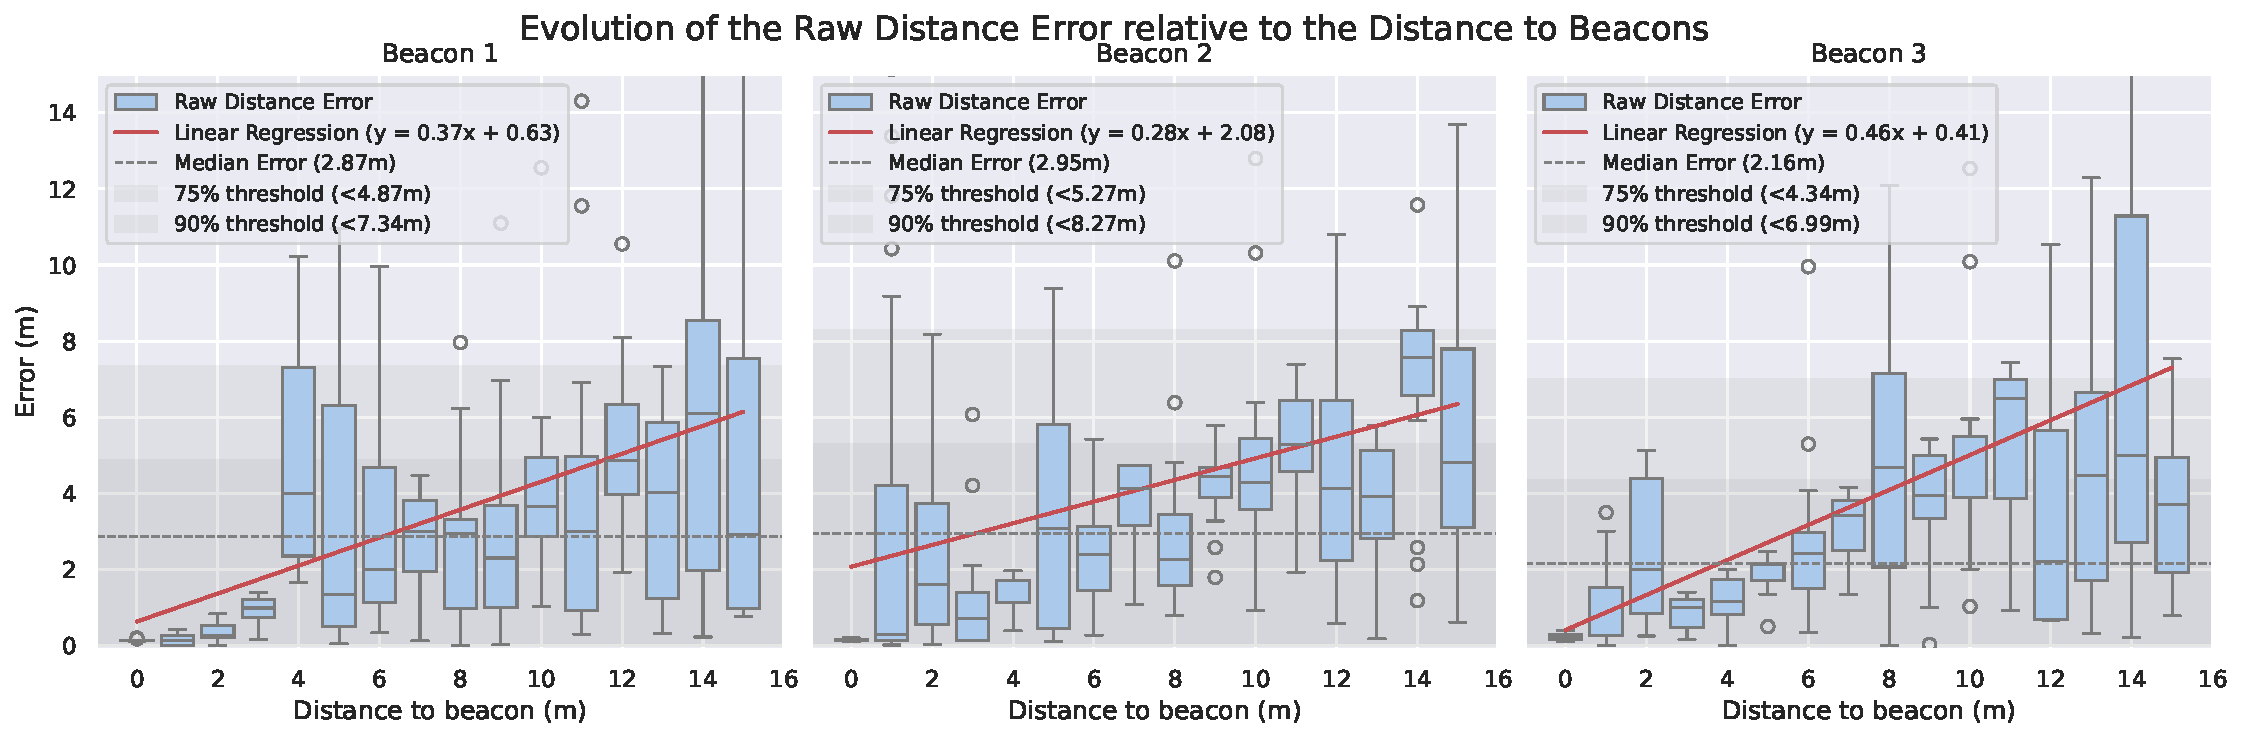
\includegraphics[width=\linewidth]{assets/beacon-dist-raw-error-by-beacon.pdf}
    \caption{Variation in Raw Distance Error relative to Distance from Beacons}
    \label{fig:beacon-dist-raw-error}
\end{figure}

\begin{figure}[h]
    \centering
    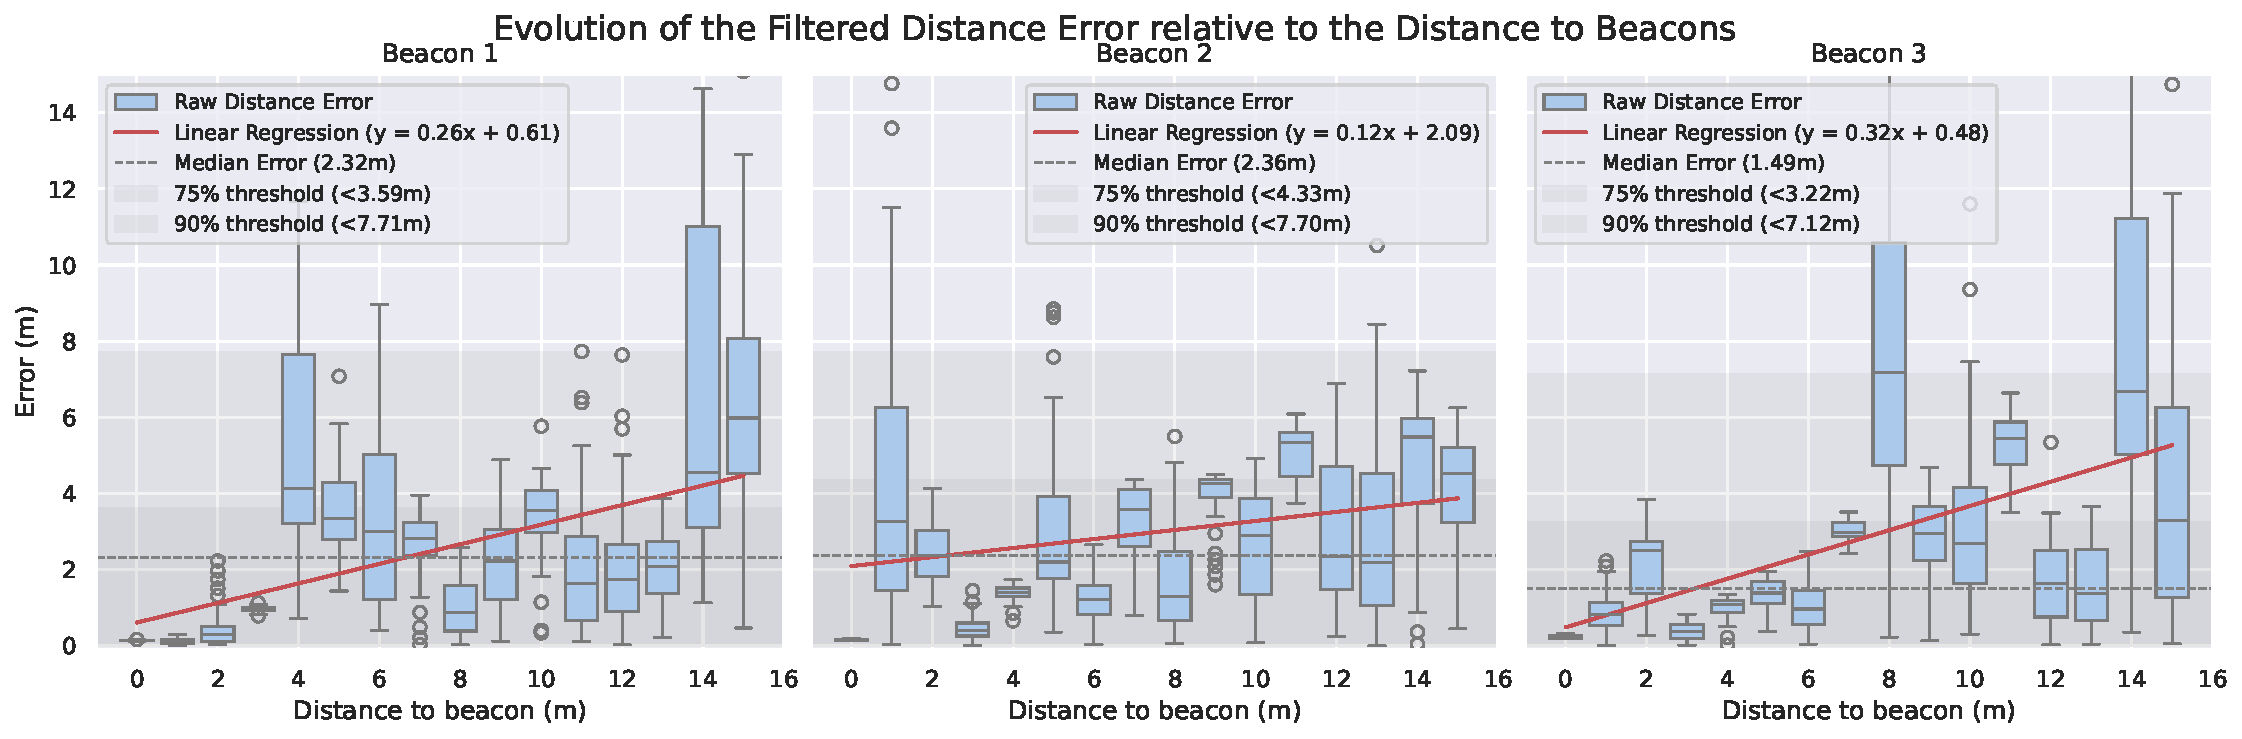
\includegraphics[width=\linewidth]{assets/beacon-dist-filtered-error-by-beacon.pdf}
    \caption{Variation in Filtered Distance Error relative to Distance from Beacons}
    \label{fig:beacon-dist-filtered-error}
\end{figure}



